\section{Durchführung}
\label{sec:Durchführung}

Die verwendete Apperatur ist in Abbildung ... schematisch dargestellt. Sie besteht aus 
einer Spannvorrichtung in Punkt A sowie zwei Auflagepunkten A und B, die %dong 
cm voneinander entfernt sind.
Nun gibt es zwei vertikal fest intergrierte Messvorichtungen, die in horizontaler Richtung 
verschiebbar sind.
\begin{figure}
    \centering
    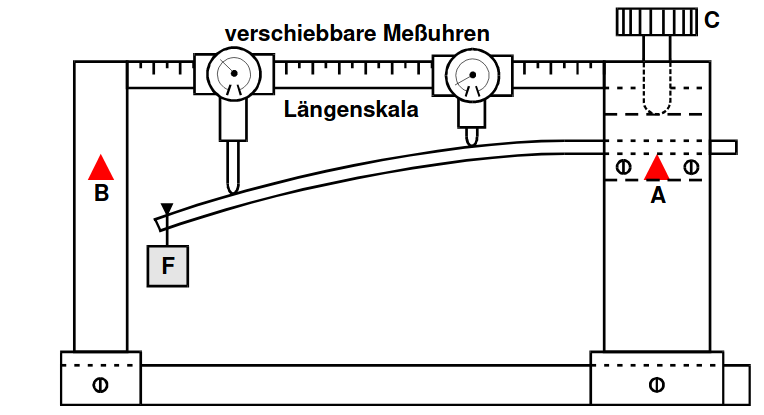
\includegraphics[scale=0.5]{panierte Austern.png}
    \caption{Schematische Darstellung einer Apparatur zur Vermessung elastisch gebogener Stäbe}
    \label{fig:backfisch}
\end{figure}

\subsection{Einseitiges Einspannen}
    Mittels der Spannvorrichtung an Punkt A werden zwei Stäbe verschiedenen Materials
    eingespannt. Um Fehlerquellen wie Vorbiegung des Stabes oder eine nicht parallele
    Ausrichtung der Messgeräte vorzubeugen, wird jeweils die Differenz der Auslenkung
    bei Normalzustand und im Zustand mit angehängtem Gewicht gemessen.\\
    Bei der ersten Messreihe mit einem viereckigen Stab wird in einer Entfernung von %dong
    cm ein Gewicht von %dong kg befestigt.
    Bei der ersten Messreihe mit einem viereckigen Stab wird in einer Entfernung von %dong
    cm ein Gewicht von %dong kg befestigt.
    Die Messwerte wurden in der Nähe der Einspannung im 5 cm Abstand und in der Nähe
    des Gewichtes im 2 cm Abstand genommen.


\subsection{Beidseitige Auflage}
    Die zu untersuchende Probe wird auf den Fußpunkten A und B gelagert. 
    

    Die Messwerte wurden in der Nähe der Einspannung im 5 cm Abstand und in der Nähe
    des Gewichtes im 2 cm Abstand genommen.